\begin{figure}
    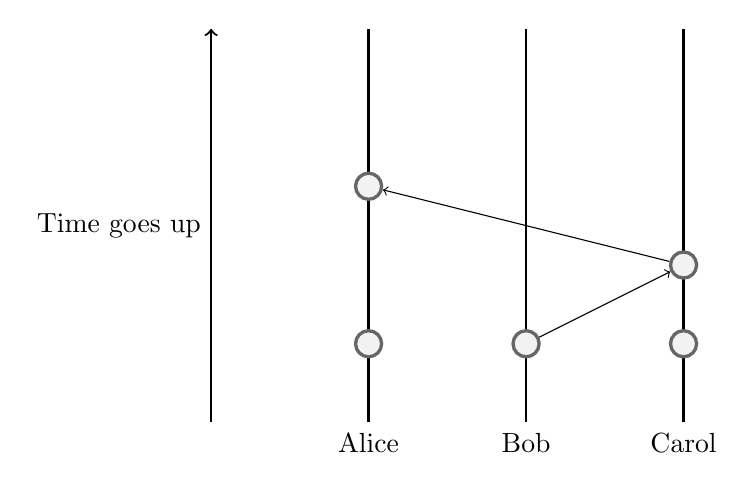
\begin{tikzpicture}[
        roundnode/.style={circle, draw=black!60, fill=black!5, very thick},
        ]

        % Lines
        \draw[thick,->] (0,0) -- (0,2.5) node[anchor=east] {Time goes up} -- (0,5);
        % Alice
        \draw[thick] (2,0) node[anchor=north] {Alice} -- (2,5);
        % Bob
        \draw[thick] (4,0) node[anchor=north] {Bob} -- (4,5);
        % Carol
        \draw[thick] (6,0) node[anchor=north] {Carol} -- (6,5);

        % Nodes
        \node[roundnode] (a1) at (2,1) { };
        \node[roundnode] (b1) at (4,1) { };
        \node[roundnode] (c1) at (6,1) { };
       
        % Gossips
        \node[roundnode] (c2) at (6,2) { };
        \node[roundnode] (a3) at (2,3) { };

        % Bob talks to Carol
        \draw[->] (b1) -- (c2);
        
        % Carol talks to Alice
        \draw[->] (c2) -- (a3);

    \end{tikzpicture}

    \label{fig:hashgraph}
    \caption{
        A simple example of how hashgraph spreads information via gossip.
        Bob gossips randomly to Carol, then Carol gossips randomly to Alice. By the end of the process,
        Alice would have known what Bob and Carol spoke about without talking to Bob directly.
    }
\end{figure}
